% \begin{figure}[t]
% % 	\centering
% % 	\hspace{-0.7in}
% 	\subfloat[Markov model from \cite{storagecharacterization}]{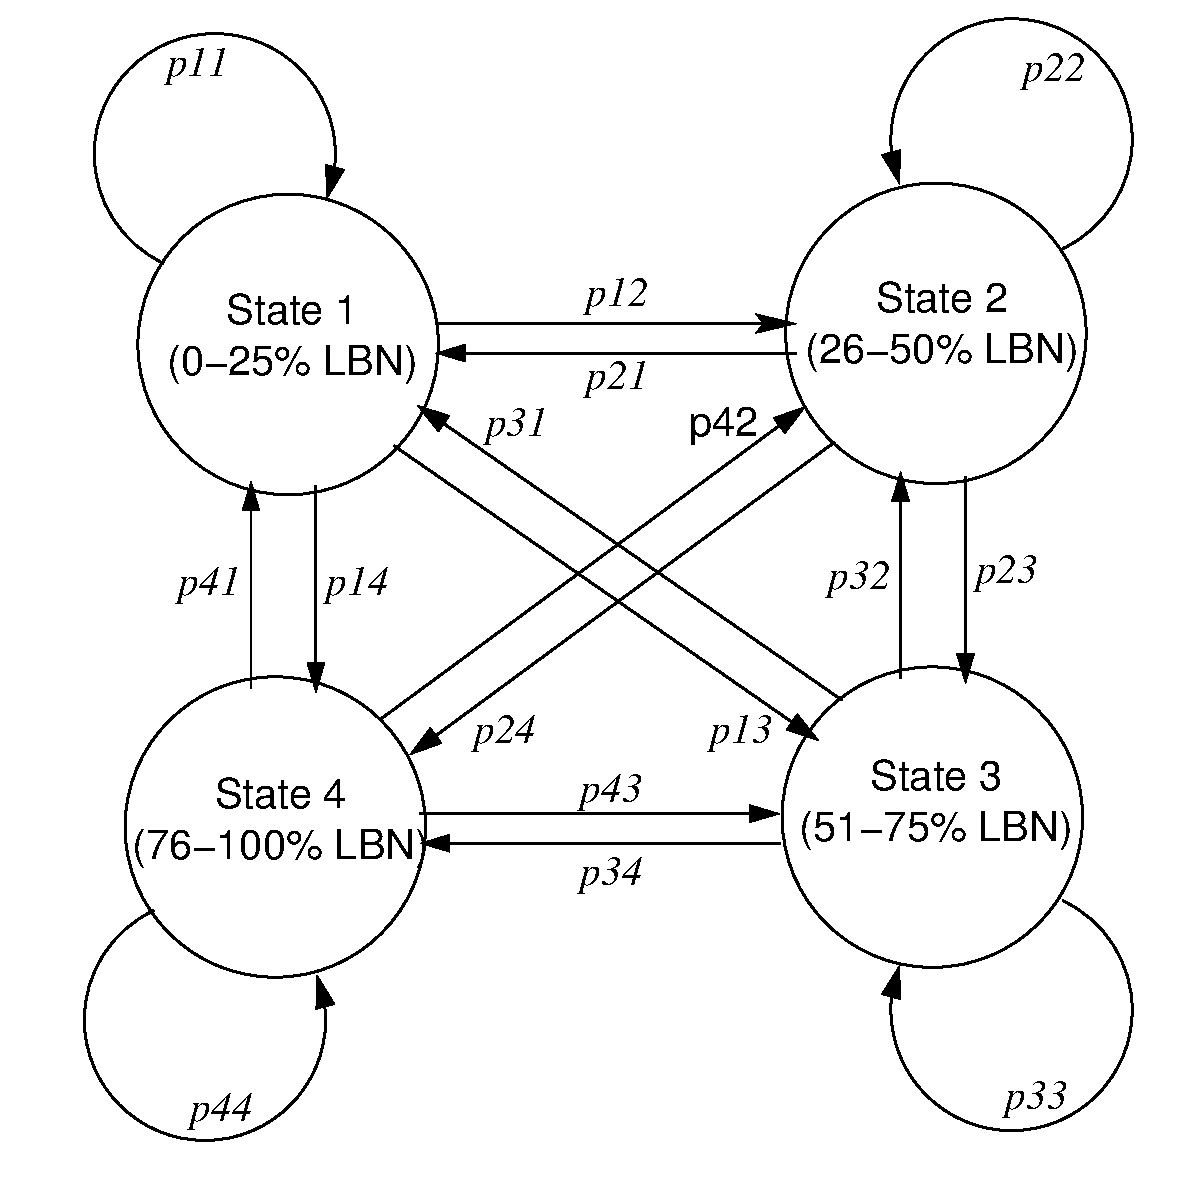
\includegraphics[scale=0.55]{presyn-figures/storagecharacterization.pdf}} \\
% 	\subfloat[Hierarchical Markov model from \cite{storagereplay,storagemodeling,decoupling-dc-studies}]{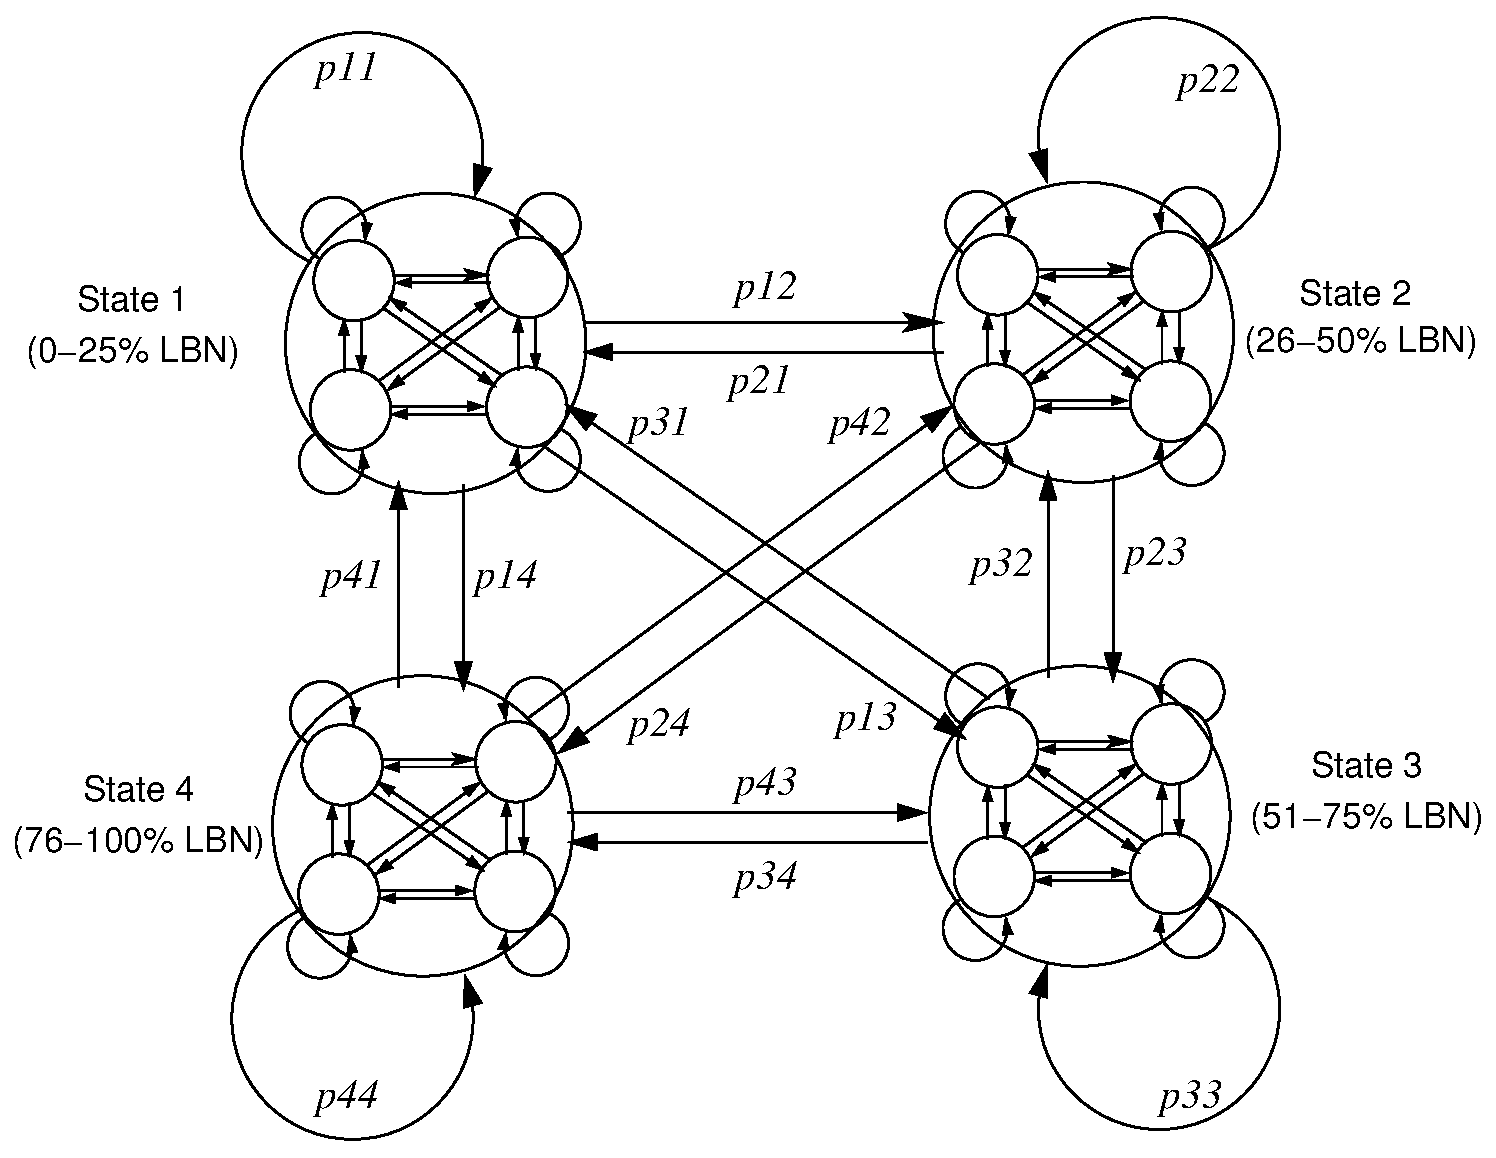
\includegraphics[scale=0.55]{presyn-figures/decoupling-dc-studies.pdf}}
% 	\caption{Using Markov models to capture the block accessed distribution~\cite{storagecharacterization, storagemodeling, storagereplay, decoupling-dc-studies}}
% 	\label{fig:storagecharacterization}
% \end{figure}

\begin{figure}[t]
	\centering
	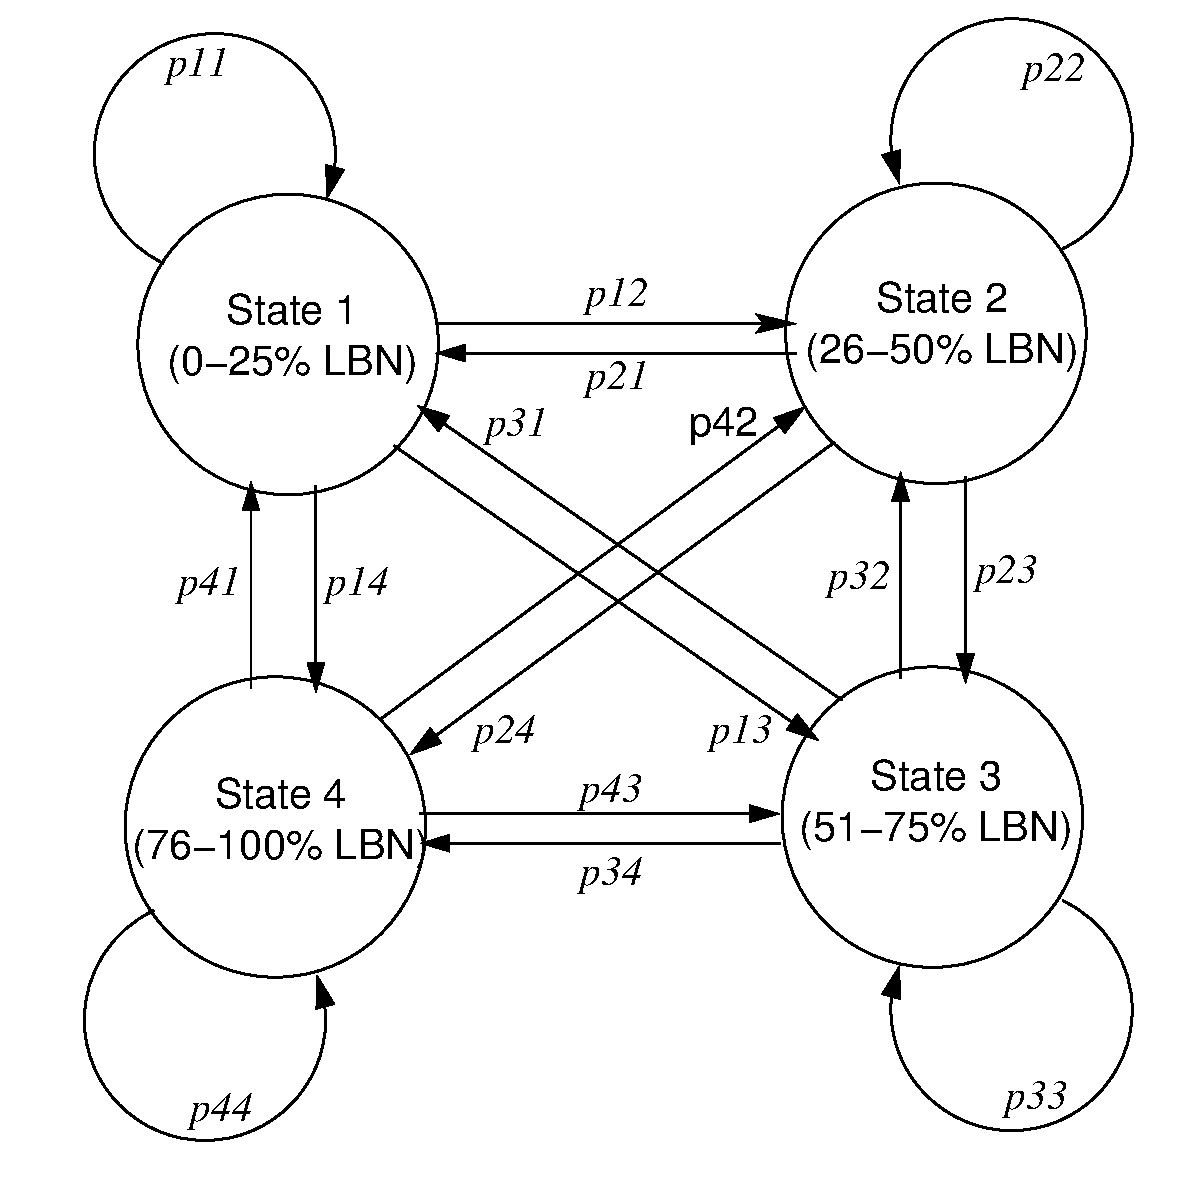
\includegraphics[scale=0.4]{presyn-figures/storagecharacterization.pdf}
	\caption{Markov model from \cite{storagecharacterization}: 
		Each arrow \textit{pij} represents probability of transition from one LBN 
			range (state \textit{i}) to itself or another (state \textit{j})}
	\label{fig:storagecharacterization}
\end{figure}


Recently, there has been significant research momentum in the direction
of surveying existing benchmarks and datasets to determine whether
enough realistic datasets or workloads are available for faithful
comparison and evaluation of competing storage optimization 
techniques~\cite{generating-datasets}.
In particular, the fields of I/O performance benchmarking as well as
storage deduplication characterization have been found wanting
with regards to availability of realistic benchmarks and datasets.
In this section, we make the case that there is significant
literature in the areas of realistic benchmark generation for 
network~\cite{echo} and 
storage I/O performance~\cite{storagecharacterization, storagemodeling,
storagereplay, flexi-replay, decoupling-dc-studies,
case-for-nas-benchmarks, jump-based-synthetic, distiller} as well as storage deduplication
evaluation~\cite{generating-datasets}, but none in the area of I/O deduplication. 

Basically, 
the I/O trace characterization and benchmark generation efforts 
focus on the request inter-arrival times as well as the spatial
and temporal locality of the access traces whereas the storage
deduplication benchmark generation effort focusses on modeling
the content duplication across temporal snapshots of the same
dataset. On the other hand, the requirement for I/O deduplication
benchmarks is a merging of the above two types of work, such 
that both the spatial/temporal locality aspects as well as
the duplicate content aspect be characterized and captured 
in the benchmark realistically. In the rest of this section,
we describe the existing work in realistic benchmark generation
under each of the categories of (i)~Storage I/O, 
(ii)~Network I/O activity, 
(iii)~File system metadata,
and
(iv)~Storage data deduplication.




\subsection{Generating realistic storage I/O performance benchmarks}
The generation of realistic I/O performance benchmarks
has received considerable attention in recent literature~\cite{storagecharacterization, storagemodeling,
storagereplay, flexi-replay, decoupling-dc-studies,
jump-based-synthetic, distiller}. 
The work in~\cite{storagecharacterization}
builds a Markov model to capture \textit{spatial locality},
with each state representing one-quarter of the 
block address range (called logical block number range or LBN range) 
and each transition representing
the probability of transitioning from one LBN range to another. The idea
is that due to the spatial nature of the workload, most of the
transitions would stay within the same state and the probabilities
of transitioning out of one state to another would be quite low. 
Thus, a request stream is perceived as a state machine 
which transitions between LBN ranges with certain probabilities.


Fig.~\ref{fig:storagecharacterization} is a reproduction of
the Markov model built in \cite{storagecharacterization}, and as
can be seen, the model has 4 states and 16 transitions between
the states. The probability of each transition in this model
is determined by characterizing real-world traces, and could
be workload-specific (i.e., dependent on the type of workload
that needs to be captured by the model). The traces used were
for web services like a message store for an email service, 
image tile storage for a large-scale geo-mapping service, and 
a blob storage service which hosted huge amounts of user-generated
content~\cite{storagecharacterization}.

\begin{figure}[t]
	\centering
	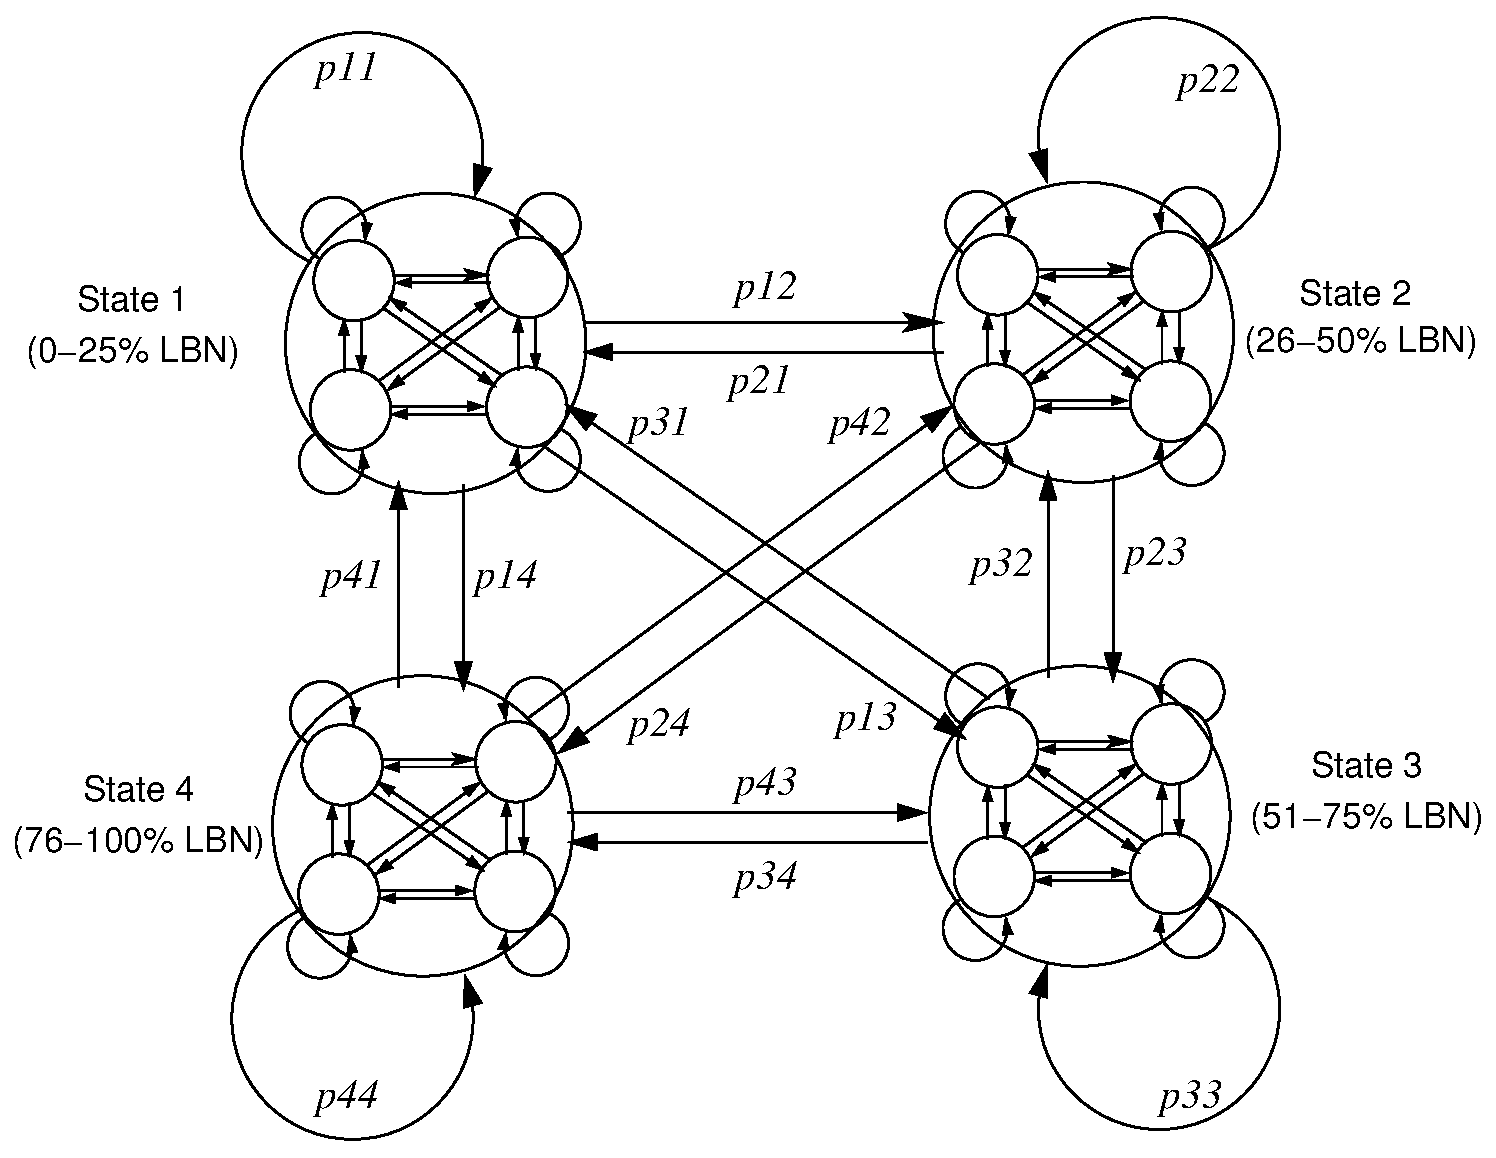
\includegraphics[scale=0.5]{presyn-figures/decoupling-dc-studies.pdf}
	\caption{Markov model from \cite{decoupling-dc-studies}: Each arrow \textit{pij} represents 
		probability of transition from one LBN
	range (state \textit{i}) to itself or another (state \textit{j}). Also, each state \textit{i}
	is further divided into 4 sub-states each, having internal transition probabilities as well.}
	\label{fig:decoupling-dc-studies}
\end{figure}


The work in~\cite{storagereplay, storagemodeling, decoupling-dc-studies}
builds on top of the above Markov model idea by building a hierarchical
Markov model such that each of the above states is further divided 
into 4 finer granularity states. For example, the LBN range
0-25\% from Fig.~\ref{fig:storagecharacterization} is broken
into 4 sub-ranges like 0-6.25\%, 6.25-12.5\%, 12.5-18.75\% 
and 18.75-25\%. Pictorially, the hierarchical Markov looks as
depicted in Fig.~\ref{fig:decoupling-dc-studies}, although
the inner states have not been marked with all the LBN sub-ranges therein.

Representing the storage I/O model as a hierarchical Markov model
enables to represent information of a finer granularity than \cite{storagecharacterization}.
Thus, the two level diagram has a total of 16 states and 76 transitions,
which are once again parameterized using a thorough characterization
of available real-world storage I/O traces.

The work in \cite{jump-based-synthetic} claims that to characterize
and recreate a realistic storage I/O workload, it is necessary to not
only capture the block accessed distribution, but also the jump distance
distribution. In view of this, the approach proposed in \cite{jump-based-synthetic}
is to transform the synthetic trace generation problem into the
Hamiltonian Path problem, and then to apply a brute-force, depth-first
search to find a Hamiltonian path (this path is expected to have the
same jump distance characteristics as the original trace). 
However, if a complete Hamiltonian
Path is not found, approximation techniques are used to construct 
the access pattern. The evaluation therein shows that if the
trace to be generated needs to have less than 150 I/O requests, only
then this brute-force approach is able to find complete Hamiltonian
paths\textemdash{}in most other cases, the algorithm is forced to rely on
the latter approximation techniques. 

The work in \cite{distiller} hypothesizes that although synthetic workloads
are flexible and easy to obtain, the challenge is that synthetic
workloads are accurate only if they share certain key properties
with the original production workload(s). The unfortunate aspect
here is that we do not know which properties are ``key'' for
any given workload or storage system. Thus, regarding the selection
of key properties for workload characterization
and generation, the work in \cite{distiller} presents a tool
called \texttt{Distiller} that can automatically identify
them using an iterative trial-and-error method. As input, the
\texttt{Distiller} tool needs a library of workload attributes, 
from which it picks one additional attribute at each iteration,
and checks whether the chosen set of attributes is representative
enough of the given workload. If so, the modeling is done and
if not, it chooses one more attribute in the next iteration
and so on until a realistic representation is achieved.

\subsection{Realistic network activity modeling and benchmark generation}
The work in \cite{echo} presents a modeling scheme called ECHO, which 
captures the temporal and spatial behaviour of network traffic in
large-scale datacenter applications. Two models are built, wherein
the first is a distribution-fitting model (called the \textit{single-server temporal
model}) that generates per-server
network traffic and the second is a Markov chain model (called the \textit{system-wide
spatial model}) that captures
server-to-server interactions. 

The single-server temporal model of \cite{echo} consists of using
a network trace as an input and identifying known distributions\textemdash{}Gaussian,
Poisson, Zipf, etc\textemdash{}in the network activity pattern. The output 
mathematical expression from this model would be a superposition of
multiple known distributions such that sampling of this composite
distribution allows to generate network activity patterns that have
similar temporal patterns as the ones present in the original trace.
However, this method captures the network activity only for
individual servers and can not address server-to-server activity
patterns or network traffic across sets of machines.

\begin{figure}[t]
	\centering
	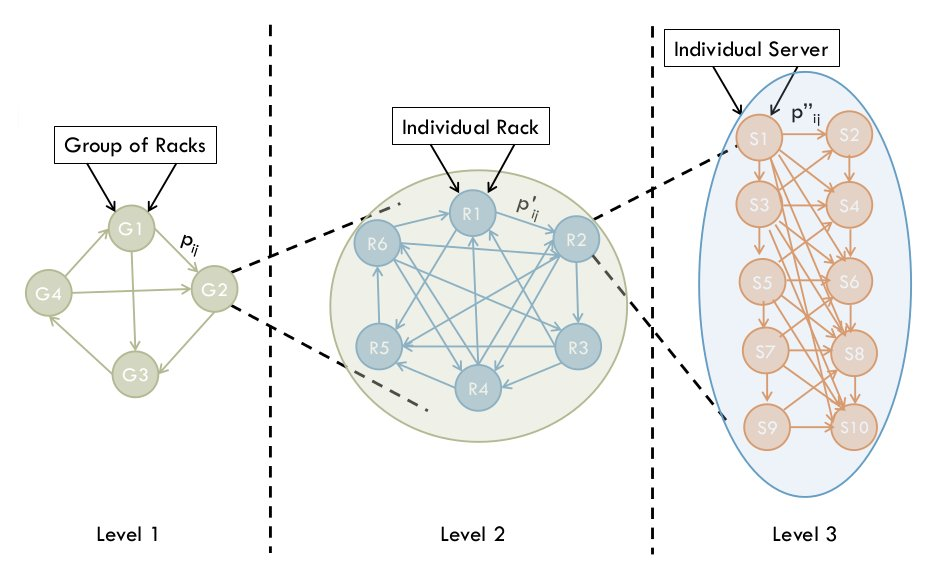
\includegraphics[scale=0.4]{presyn-figures/echo.jpg}
	\caption{Schematic of the hierarchical spatial Markov chain model~\cite{echo}}
	\label{fig:echo}
\end{figure}

The second model developed in \cite{echo} is a hierarchical Markov
chain model which captures the network activity patterns for
individual servers, across servers within a rack, as well as
across racks within a group of racks. Fig.~\ref{fig:echo} is 
a lifted reproduction from \cite{echo} of the schematic of
the hierarchical spatial Markov chain model. 
As can be seen, this model is hierarchical, and 
the level of detail in the model can be adjusted according to the
requirements of each application.

\subsection{Generating realistic file system benchmarks}
Similar to the quest in \cite{distiller} regarding the key properties 
of a given workload, the work in \cite{impressions} is motivated by
the key properties needed to realistically represent a file system
image. The claim therein, is that, depending on the workload to
be emulated or evaluated, the file system image to be used may
need different levels of detail. For example, a data mirroring
scheme like RAID or a system that takes full backups would be
independent of both metadata and content of the filesystem.
On the other extreme, a desktop search engine's performance
would depend on both the metadata and the exact content of
the file system on which it operates.

Although the work in \cite{impressions} does not address the evaluation
or analysis of deduplication techniques, the framework (called \textit{Impressions})
presented therein would be useful to capture the content profile
of any real file system such that deduplication techniques can
be evaluated over it~\cite{generating-datasets}.

\subsection{Generating realistic storage deduplication benchmarks} 
To justify the creation of benchmarks for storage deduplication, the work in
\cite{generating-datasets} claims that the benchmark or datasets should be
such that they should be :-
\begin{enumerate}
		\singlespacing
	\item Sufficiently large
	\item Having controllable characteristics
	\item Easy to distribute to other researchers
	\item Easily accessible or reproducible by other researchers
	\item Realistic
\end{enumerate}

The requirement of ``realistic'' datasets is straight-forward\textemdash{}unless the
dataset is realistic, there is no way to judge whether any proposed 
technique is useful in the real world. 
However, if the dataset is ``realistic'' because it contains proprietary
or private information, then the owner of the dataset may be reluctant to
make the dataset publicly available. Further, the requirement
that the dataset is sufficiently large, is also at crossroads with the 
requirement that the dataset be easily accessible to other researchers,
because larger the dataset, tougher the task of hosting and maintaining
it online.

Due to above conflicting requirements, the work in \cite{generating-datasets}
suggests a framework which involves capturing the important characteristics
of a real-world workload into a model which can be represented with a much
smaller storage footprint than the actual workload, and hence can be easily
distributed across research groups. The work in \cite{generating-datasets}
generates benchmarks which capture the changes in file system across multiple
snapshots (referred to as \textit{mutation}) along-with its content 
representation, using a combination of a 
Markov model and a multi-dimensional distribution model.

The work in \cite{dedis} presents DEDISbench, a realistic storage
deduplication benchmark. 
The I/O generation framework in DEDISbench consists of two
components: (i) Access pattern generator, and (ii) Content generator.
The access pattern generator can generate sequential, uniform-random
or random-with-hotspots accesses depending on user choice.
The random-with-hotspots access pattern
uses TPC-C NURand function to simulate
access hotspots in write requests\textemdash{}access hotspot implies that
a few blocks will be accessed multiple times while other blocks may 
only be accessed once each. 
If the request is a write request, the
content generator generates the random content to be written to 
the specified block, based on an input distribution of 
duplicates.
A tool called DEDISgen is also
presented~\cite{dedis}, which can be used to compute the cumulative
distributions of block accesses for a real filesystem such that 
this distribution can be used as an input to DEDISbench for generating
the realistic benchmarks for storage deduplication.

Since our requirement is to evaluate read I/O deduplication techniques,
and not storage deduplication, hence to use DEDISbench, we would need
to tweak it such that access hotspots are created for read accesses
as well, and not just for write requests. 
Moreover, the realistic nature of not only the content in the 
filesystem (i.e., on storage) but also the content in the 
read I/O (i.e., in I/O traces)
needs to be captured. Specifically, DEDISbench uses the duplicate
distribution to guide the content generation for write requests.
We need the read access hotspots to also be similarly guided by
a duplicate distribution of content present in real I/O 
traces\textemdash{}basically
to capture the dual metrics of \textit{sharing factor} and 
\textit{occurrence factor} of every content in the trace.
\\
\\
Based on the above surveyed literature, we conclude that there are no
realistic benchmarking tools or trace generation frameworks that can
be used for evaluation of I/O deduplication techniques. Thus, for the 
evaluation of such techniques, researchers need to either collect multiple
production workload traces for their own research, or create frameworks
that can synthesize realistic I/O traces along-with content representation.
% In the next sub-section, we present some potential ideas for building
% controllable synthetic traces for I/O deduplication analysis, with 
% the caveat that actually building such traces and using them for 
% evaluation would again require access to certain realistic workloads,
% and hence is beyond the scope of this thesis.
% 
% \subsection{Proposed approach for generating controllable, realistic I/O workloads with duplicate content}
% details pending
